\documentclass[tikz,border=10pt]{standalone}
\usetikzlibrary{arrows.meta, positioning, calc, decorations.pathreplacing}
\usepackage{amssymb}

\begin{document}
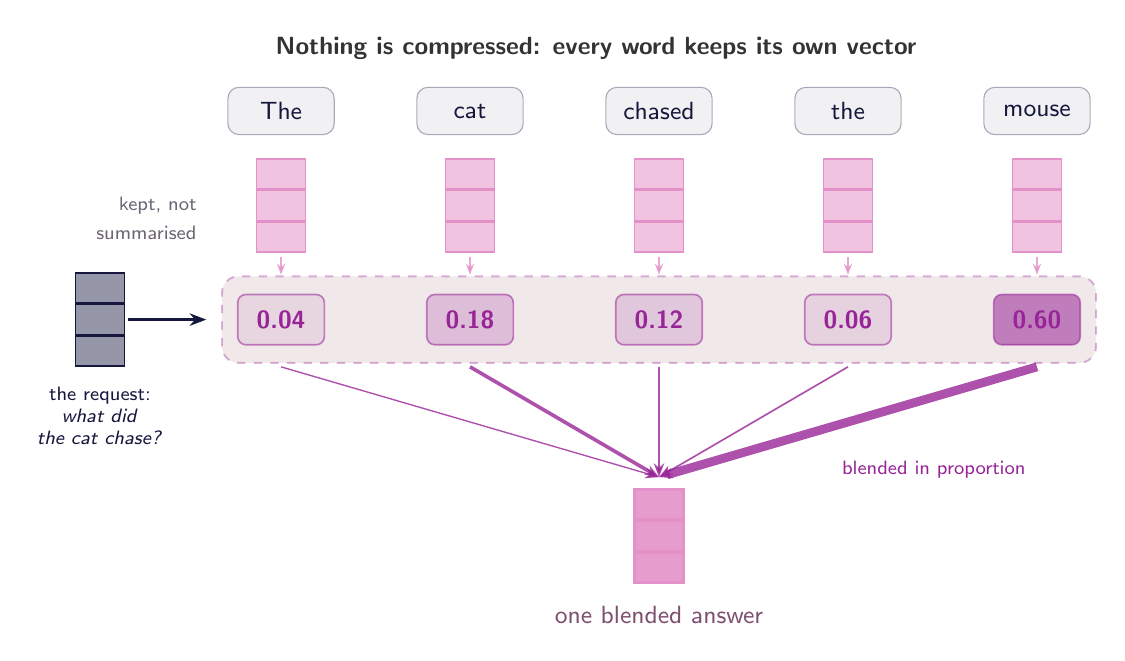
\begin{tikzpicture}[
    every node/.style={font=\sffamily},
]

% ---------------------------------------------------------------- colours
\definecolor{c1}{HTML}{15173D}   % tokens, and the request (the query role)
\definecolor{c2}{HTML}{982598}   % the match scores (the operative step)
\definecolor{c3}{HTML}{E491C9}   % the per-word vectors, and the answer
\definecolor{c4}{HTML}{F1E9E9}   % the matching band
\definecolor{axiscolor}{HTML}{333333}
\definecolor{labelcolor}{HTML}{6B6472}

% ---------------------------------------------------------------- styles
\tikzset{
    word/.style={
        rectangle, rounded corners=4pt, minimum width=1.35cm,
        minimum height=0.6cm, inner xsep=4pt,
        draw=c1, draw opacity=0.35, fill=c1, fill opacity=0.06,
        text=c1, text opacity=1, font=\sffamily\small,
    },
    vcell/.style={
        rectangle, minimum width=0.62cm, minimum height=0.38cm,
        draw=c3, line width=0.5pt, fill=c3, fill opacity=0.55,
    },
    qcell/.style={
        rectangle, minimum width=0.62cm, minimum height=0.38cm,
        draw=c1, line width=0.5pt, fill=c1, fill opacity=0.45,
    },
    ocell/.style={
        rectangle, minimum width=0.62cm, minimum height=0.38cm,
        draw=c3, line width=0.9pt, fill=c3, fill opacity=0.9,
    },
}

% ================================================================
% GEOMETRY
%   word columns   x = 0.6, 3.0, 5.4, 7.8, 10.2
%   word labels    y = 6.7
%   word vectors   y = 5.9 / 5.5 / 5.1
%   matching band  y = 3.55 .. 4.55
%   answer         y = 1.7 / 1.3 / 0.9, centred on x = 5.4
%   the request    x = -1.7
% ================================================================

\node[font=\sffamily\small\bfseries, text=axiscolor] at (4.6, 7.5)
    {Nothing is compressed: every word keeps its own vector};

% ---------------------------------------------------------------- the words
\node[word] (w1) at (0.6, 6.7) {The};
\node[word] (w2) at (3.0, 6.7) {cat};
\node[word] (w3) at (5.4, 6.7) {chased};
\node[word] (w4) at (7.8, 6.7) {the};
\node[word] (w5) at (10.2, 6.7) {mouse};

\foreach \x/\n in {0.6/1, 3.0/2, 5.4/3, 7.8/4, 10.2/5} {
    \foreach \k in {0,1,2} {
        \node[vcell] at (\x, 5.9 - \k*0.4) {};
    }
    \draw[-{Stealth[length=4pt]}, line width=0.8pt, c3, opacity=0.8]
        (\x, 4.85) -- (\x, 4.62);
}

\node[font=\sffamily\scriptsize, text=labelcolor, anchor=east] at (-0.35, 5.5)
    {kept, not};
\node[font=\sffamily\scriptsize, text=labelcolor, anchor=east] at (-0.35, 5.15)
    {summarised};

% ---------------------------------------------------------------- the request
\foreach \k in {0,1,2} {
    \node[qcell] at (-1.7, 4.45 - \k*0.4) {};
}
% anchor=north so the label grows downward. Centred on its own midpoint it
% grows upward too, and the first line collides with the bottom cell above.
\node[font=\sffamily\scriptsize, text=c1, align=center, anchor=north]
    at (-1.7, 3.32)
    {the request:\\\emph{what did}\\\emph{the cat chase?}};

\draw[-{Stealth[length=6pt]}, line width=1.1pt, c1]
    (-1.35, 4.05) -- (-0.35, 4.05);

% ---------------------------------------------------------------- matching
\fill[c4, rounded corners=6pt] (-0.15, 3.5) rectangle (10.95, 4.6);
\draw[c2, opacity=0.35, dashed, line width=0.7pt, rounded corners=6pt]
    (-0.15, 3.5) rectangle (10.95, 4.6);

% score boxes: fill opacity carries the weight, so the winner is visible
% before any number is read
\foreach \x/\a/\o in {0.6/0.04/0.10, 3.0/0.18/0.22, 5.4/0.12/0.17,
                      7.8/0.06/0.12, 10.2/0.60/0.55} {
    \fill[c2, opacity=\o, rounded corners=3pt]
        (\x-0.55, 3.73) rectangle (\x+0.55, 4.37);
    \draw[c2, opacity=0.55, rounded corners=3pt, line width=0.6pt]
        (\x-0.55, 3.73) rectangle (\x+0.55, 4.37);
    \node[font=\sffamily\small\bfseries, text=c2] at (\x, 4.05) {\a};
}

% the "every word reports how well it answers" line lives in the figcaption:
% inside the figure it sits on top of the converging arrows

% ---------------------------------------------------------------- blending
% arrow weight is proportional to the score, so the picture says the same
% thing as the numbers
\foreach \x/\w in {0.6/0.5, 3.0/1.3, 5.4/0.95, 7.8/0.6, 10.2/3.2} {
    \draw[-{Stealth[length=5pt]}, line width=\w pt, c2, opacity=0.8]
        (\x, 3.45) -- (5.4, 2.05);
}

\node[font=\sffamily\scriptsize, text=c2, anchor=west] at (7.6, 2.15)
    {blended in proportion};

% ---------------------------------------------------------------- the answer
\foreach \k in {0,1,2} {
    \node[ocell] at (5.4, 1.7 - \k*0.4) {};
}
\node[font=\sffamily\small, text=c3!55!black] at (5.4, 0.3)
    {one blended answer};

\end{tikzpicture}
\end{document}
